%!TeX root=../pridetop.tex
\chapter[Chapter \thechapter]{}
	

\begin{figure}[t!]
\centering
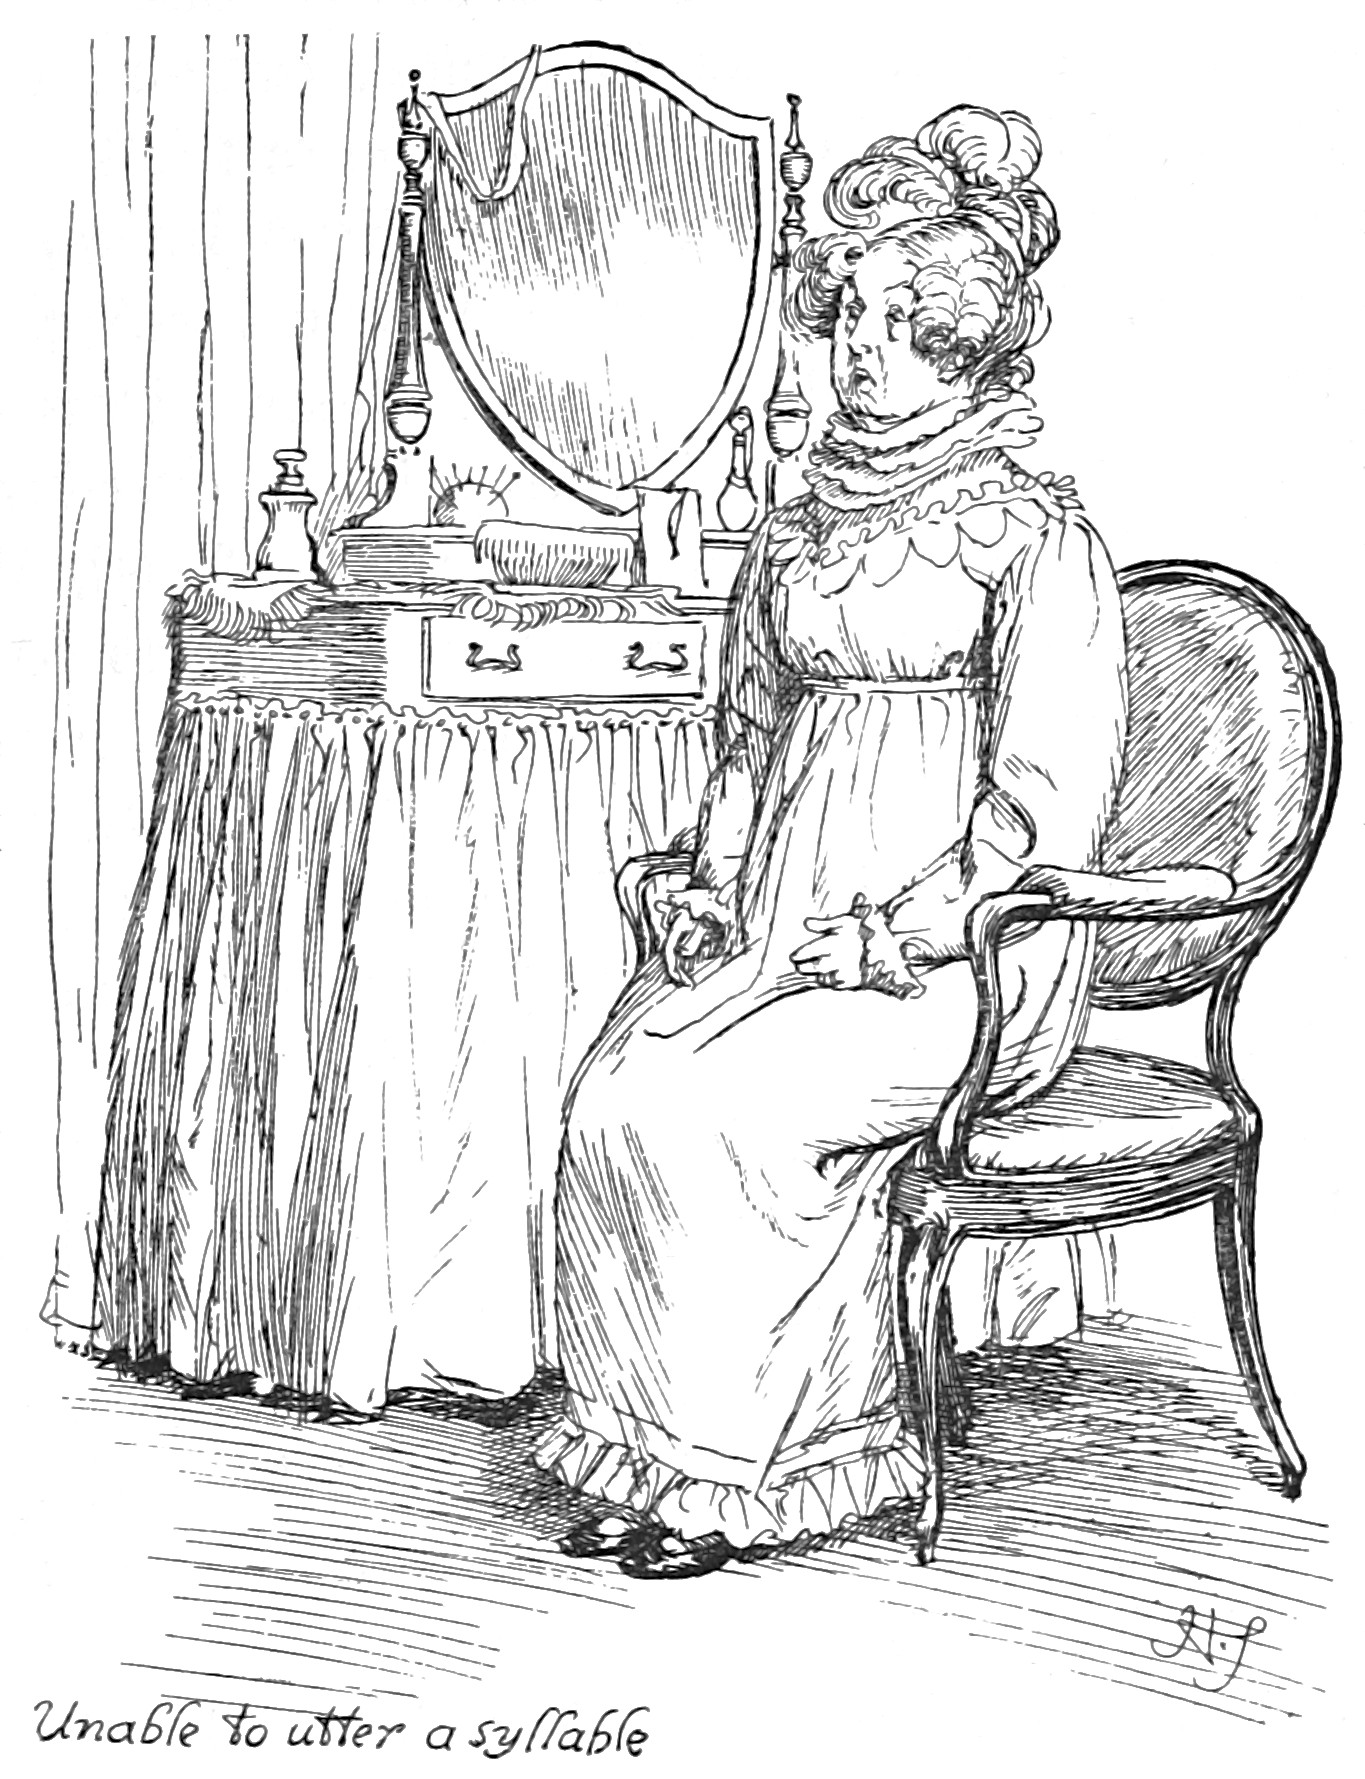
\includegraphics[width=.7\linewidth]{59top}
\captionlistentry{Unable to utter a syllable}
\end{figure}


\lettrine[lines=6,image=true,ante=`]{initials/chap59m}{y} dear Lizzy, where can you have been walking to?' was a question which Elizabeth received from Jane as soon as she entered the room, and from all the others when they sat down to table. She had only to say in reply, that they had wandered about till she was beyond her own knowledge. She coloured as she spoke; but neither that, nor anything else, awakened a suspicion of the truth.

The evening passed quietly, unmarked by anything extraordinary. The acknowledged lovers talked and laughed; the unacknowledged were silent. Darcy was not of a disposition in which happiness overflows in mirth; and Elizabeth, agitated and confused, rather \textit{knew} that she was happy than \textit{felt} herself to be so; for, besides the immediate embarrassment, there were other evils before her. She anticipated what would be felt in the family when her situation became known: she was aware that no one liked him but Jane; and even feared that with the others it was a \textit{dislike} which not all his fortune and consequence might do away.

At night she opened her heart to Jane. Though suspicion was very far from Miss Bennet's general habits, she was absolutely incredulous here.

»You are joking, Lizzy. This cannot be! Engaged to Mr Darcy! No, no, you shall not deceive me: I know it to be impossible.«

»This is a wretched beginning, indeed! My sole dependence was on you; and I am sure nobody else will believe me, if you do not. Yet, indeed, I am in earnest. I speak nothing but the truth. He still loves me, and we are engaged.«

Jane looked at her doubtingly. »Oh, Lizzy! it cannot be. I know how much you dislike him.«

»You know nothing of the matter. \textit{That} is all to be forgot. Perhaps I did not always love him so well as I do now; but in such cases as these a good memory is unpardonable. This is the last time I shall ever remember it myself.«

Miss Bennet still looked all amazement. Elizabeth again, and more seriously, assured her of its truth.

»Good heaven! can it be really so? Yet now I must believe you,« cried Jane. »My dear, dear Lizzy, I would, I do congratulate you; but are you certain—forgive the question—are you quite certain that you can be happy with him?«

»There can be no doubt of that. It is settled between us already that we are to be the happiest couple in the world. But are you pleased, Jane? Shall you like to have such a brother?«

»Very, very much. Nothing could give either Bingley or myself more delight. But we considered it, we talked of it as impossible. And do you really love him quite well enough? Oh, Lizzy! do anything rather than marry without affection. Are you quite sure that you feel what you ought to do?«

»Oh, yes! You will only think I feel \textit{more} than I ought to do when I tell you all.«

»What do you mean?«

»Why, I must confess that I love him better than I do Bingley. I am afraid you will be angry.«

»My dearest sister, now be, \textit{be} serious. I want to talk very seriously. Let me know everything that I am to know without delay. Will you tell me how long you have loved him?«

»It has been coming on so gradually, that I hardly know when it began; but I believe I must date it from my first seeing his beautiful grounds at Pemberley.«

Another entreaty that she would be serious, however, produced the desired effect; and she soon satisfied Jane by her solemn assurances of attachment. When convinced on that article, Miss Bennet had nothing further to wish.

»Now I am quite happy,« said she, »for you will be as happy as myself. I always had a value for him. Were it for nothing but his love of you, I must always have esteemed him; but now, as Bingley's friend and your husband, there can be only Bingley and yourself more dear to me. But, Lizzy, you have been very sly, very reserved with me. How little did you tell me of what passed at Pemberley and Lambton! I owe all that I know of it to another, not to you.«

Elizabeth told her the motives of her secrecy. She had been unwilling to mention Bingley; and the unsettled state of her own feelings had made her equally avoid the name of his friend: but now she would no longer conceal from her his share in Lydia's marriage. All was acknowledged, and half the night spent in conversation.

»Good gracious!« cried Mrs Bennet, as she stood at a window the next morning, »if that disagreeable Mr Darcy is not coming here again with our dear Bingley! What can he mean by being so tiresome as to be always coming here? I had no notion but he would go a-shooting, or something or other, and not disturb us with his company. What shall we do with him? Lizzy, you must walk out with him again, that he may not be in Bingley's way.«

Elizabeth could hardly help laughing at so convenient a proposal; yet was really vexed that her mother should be always giving him such an epithet.

As soon as they entered, Bingley looked at her so expressively, and shook hands with such warmth, as left no doubt of his good information; and he soon afterwards said aloud, »Mrs Bennet, have you no more lanes hereabouts in which Lizzy may lose her way again to-day?«

»I advise Mr Darcy, and Lizzy, and Kitty,« said Mrs Bennet, »to walk to Oakham Mount this morning. It is a nice long walk, and Mr Darcy has never seen the view.«

»It may do very well for the others,« replied Mr Bingley; »but I am sure it will be too much for Kitty. Won't it, Kitty?«

Kitty owned that she had rather stay at home. Darcy professed a great curiosity to see the view from the Mount, and Elizabeth silently consented. As she went upstairs to get ready, Mrs Bennet followed her, saying,—

»I am quite sorry, Lizzy, that you should be forced to have that disagreeable man all to yourself; but I hope you will not mind it. It is all for Jane's sake, you know; and there is no occasion for talking to him except just now and then; so do not put yourself to inconvenience.«

During their walk, it was resolved that Mr Bennet's consent should be asked in the course of the evening: Elizabeth reserved to herself the application for her mother's. She could not determine how her mother would take it; sometimes doubting whether all his wealth and grandeur would be enough to overcome her abhorrence of the man; but whether she were violently set against the match, or violently delighted with it, it was certain that her manner would be equally ill adapted to do credit to her sense; and she could no more bear that Mr Darcy should hear the first raptures of her joy, than the first vehemence of her disapprobation.

In the evening, soon after Mr Bennet withdrew to the library, she saw Mr Darcy rise also and follow him, and her agitation on seeing it was extreme. She did not fear her father's opposition, but he was going to be made unhappy, and that it should be through her means; that \textit{she}, his favourite child, should be distressing him by her choice, should be filling him with fears and regrets in disposing of her, was a wretched reflection, and she sat in misery till Mr Darcy appeared again, when, looking at him, she was a little relieved by his smile. In a few minutes he approached the table where she was sitting with Kitty; and, while pretending to admire her work, said in a whisper, »Go to your father; he wants you in the library.« She was gone directly.

Her father was walking about the room, looking grave and anxious. »Lizzy,« said he, »what are you doing? Are you out of your senses to be accepting this man? Have not you always hated him?«

How earnestly did she then wish that her former opinions had been more reasonable, her expressions more moderate! It would have spared her from explanations and professions which it was exceedingly awkward to give; but they were now necessary, and she assured him, with some confusion, of her attachment to Mr Darcy.

»Or, in other words, you are determined to have him. He is rich, to be sure, and you may have more fine clothes and fine carriages than Jane. But will they make you happy?«

»Have you any other objection,« said Elizabeth, »than your belief of my indifference?«

»None at all. We all know him to be a proud, unpleasant sort of man; but this would be nothing if you really liked him.«

»I do, I do like him,« she replied, with tears in her eyes; »I love him. Indeed he has no improper pride. He is perfectly amiable. You do not know what he really is; then pray do not pain me by speaking of him in such terms.«

»Lizzy,« said her father, »I have given him my consent. He is the kind of man, indeed, to whom I should never dare refuse anything, which he condescended to ask. I now give it to \textit{you}, if you are resolved on having him. But let me advise you to think better of it. I know your disposition, Lizzy. I know that you could be neither happy nor respectable, unless you truly esteemed your husband, unless you looked up to him as a superior. Your lively talents would place you in the greatest danger in an unequal marriage. You could scarcely escape discredit and misery. My child, let me not have the grief of seeing \textit{you} unable to respect your partner in life. You know not what you are about.«

Elizabeth, still more affected, was earnest and solemn in her reply; and, at length, by repeated assurances that Mr Darcy was really the object of her choice, by explaining the gradual change which her estimation of him had undergone, relating her absolute certainty that his affection was not the work of a day, but had stood the test of many months' suspense, and enumerating with energy all his good qualities, she did conquer her father's incredulity, and reconcile him to the match.

»Well, my dear,« said he, when she ceased speaking, »I have no more to say. If this be the case, he deserves you. I could not have parted with you, my Lizzy, to anyone less worthy.«

To complete the favourable impression, she then told him what Mr Darcy had voluntarily done for Lydia. He heard her with astonishment.

»This is an evening of wonders, indeed! And so, Darcy did everything; made up the match, gave the money, paid the fellow's debts, and got him his commission! So much the better. It will save me a world of trouble and economy. Had it been your uncle's doing, I must and \textit{would} have paid him; but these violent young lovers carry everything their own way. I shall offer to pay him to-morrow, he will rant and storm about his love for you, and there will be an end of the matter.«

He then recollected her embarrassment a few days before on his reading Mr Collins's letter; and after laughing at her some time, allowed her at last to go, saying, as she quitted the room, »If any young men come for Mary or Kitty, send them in, for I am quite at leisure.«

Elizabeth's mind was now relieved from a very heavy weight; and, after half an hour's quiet reflection in her own room, she was able to join the others with tolerable composure. Everything was too recent for gaiety, but the evening passed tranquilly away; there was no longer anything material to be dreaded, and the comfort of ease and familiarity would come in time.

When her mother went up to her dressing-room at night, she followed her, and made the important communication. Its effect was most extraordinary; for, on first hearing it, Mrs Bennet sat quite still, and unable to utter a syllable. Nor was it under many, many minutes, that she could comprehend what she heard, though not in general backward to credit what was for the advantage of her family, or that came in the shape of a lover to any of them. She began at length to recover, to fidget about in her chair, get up, sit down again, wonder, and bless herself.

»Good gracious! Lord bless me! only think! dear me! Mr Darcy! Who would have thought it? And is it really true? Oh, my sweetest Lizzy! how rich and how great you will be! What pin-money, what jewels, what carriages you will have! Jane's is nothing to it—nothing at all. I am so pleased—so happy. Such a charming man! so handsome! so tall! Oh, my dear Lizzy! pray apologize for my having disliked him so much before. I hope he will overlook it. Dear, dear Lizzy. A house in town! Everything that is charming! Three daughters married! Ten thousand a year! Oh, Lord! what will become of me? I shall go distracted.«

This was enough to prove that her approbation need not be doubted; and Elizabeth, rejoicing that such an effusion was heard only by herself, soon went away. But before she had been three minutes in her own room, her mother followed her.

»My dearest child,« she cried, »I can think of nothing else. Ten thousand a year, and very likely more! 'Tis as good as a lord! And a special licence—you must and shall be married by a special licence. But, my dearest love, tell me what dish Mr Darcy is particularly fond of, that I may have it to-morrow.«

This was a sad omen of what her mother's behaviour to the gentleman himself might be; and Elizabeth found that, though in the certain possession of his warmest affection, and secure of her relations' consent, there was still something to be wished for. But the morrow passed off much better than she expected; for Mrs Bennet luckily stood in such awe of her intended son-in-law, that she ventured not to speak to him, unless it was in her power to offer him any attention, or mark her deference for his opinion.

Elizabeth had the satisfaction of seeing her father taking pains to get acquainted with him; and Mr Bennet soon assured her that he was rising every hour in his esteem.

»I admire all my three sons-in-law highly,« said he. »Wickham, perhaps, is my favourite; but I think I shall like \textit{your} husband quite as well as Jane's.«